\documentclass[tikz,border=5pt]{standalone}
% https://tex.stackexchange.com/q/757452/322482
\usetikzlibrary{calc,backgrounds}
\newcommand*\drawSemicircle[3][]{%
    \coordinate (mid) at ($(#2)!0.5!(#3)$);
    \draw[#1] (#2)
    let
        \p{A} = ($(#2)-(mid)$),
        \p{B} = ($(#3)-(mid)$),
        \n{cross} = {\x{A}*\y{B} - \y{A}*\x{B}},
        \n{angA} = {atan2(\y{A},\x{A})},
        \n{angB} = {atan2(\y{B},\x{B})},
        \n{R}    = {veclen(\x{A},\y{A})},
        \n{start} = {(\n{cross}>=0 ? \n{angA} : \n{angB})},
        \n{endraw} = {(\n{cross}>=0 ? \n{angB} : \n{angA})},
        \n{end} = {(\n{endraw} < \n{start} ? \n{endraw} + 360 : \n{endraw})}
    in arc[start angle=\n{start},end angle=\n{end},radius=\n{R}];
}
\newcommand*\drawinnerarc[4][]{
    % #2/#3: start/end
    % #4: radius
    \draw[orange,thick,#1] (in-#2) -- ({#2*6}:#4 cm) arc[start angle={#2*6},end angle={#3*6-3},radius=#4cm] -- ({#3*6-3}:#4cm) -- ({#3*6-3}:5.8cm) -- (out-#3);
}
\begin{document}
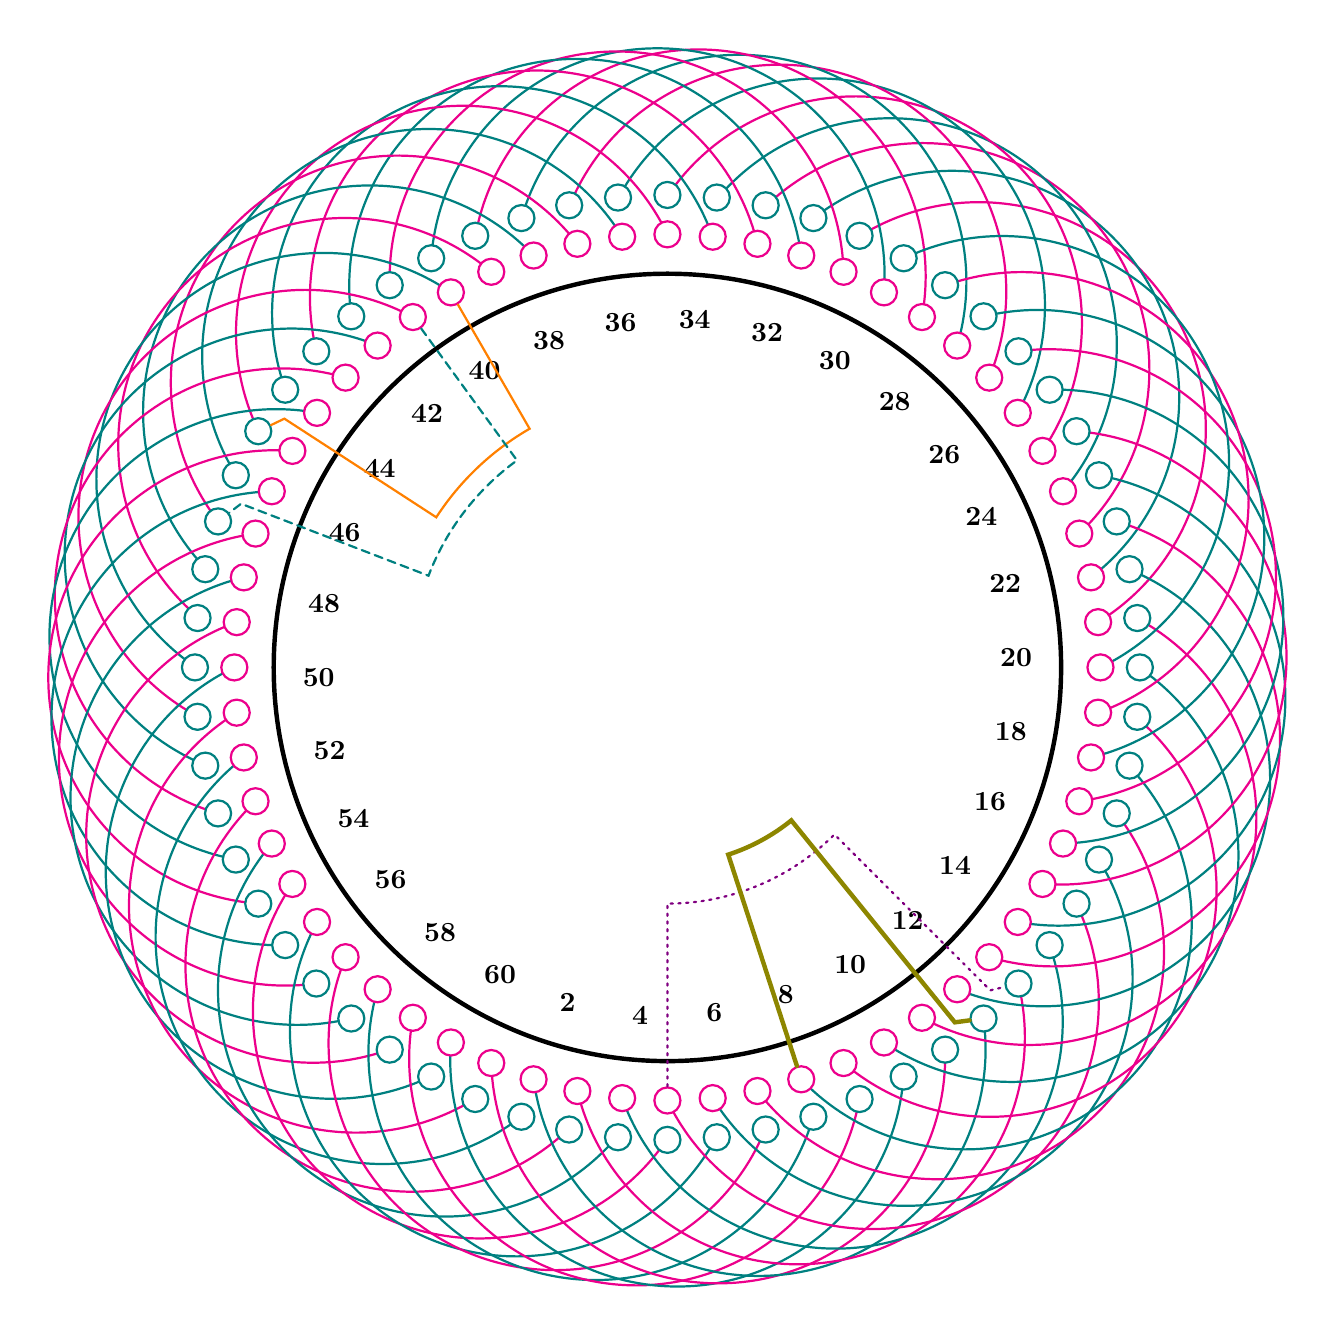
\begin{tikzpicture}[line cap=round]
    \draw[ultra thick] circle[radius=5cm];
    \foreach \x in {1,...,60}{
        \ifodd\x\else\node[label={[circle,minimum size=.5cm,inner sep=0pt,anchor=center,font=\bfseries]{\x*6}:\x}] at ({\x*6-120}:4.5cm) {};\fi
        \node[circle,fill=white,draw=magenta,thick] (in-\x) at ({\x*6}:5.5cm) {};
        \node[circle,fill=white,draw=teal,thick] (out-\x) at ({\x*6}:6cm) {};
    }
    \begin{scope}[on background layer]%
        \foreach \pstart[evaluate=\pstart as \pend using {int(mod(\pstart+9,60)+1)}] in {1,...,60}{
            \ifodd\pstart\gdef\mycolor{magenta}\else\gdef\mycolor{teal}\fi
            \drawSemicircle[thick,\mycolor]{in-\pstart}{out-\pend}
        }
    \end{scope}
\drawinnerarc{20}{25}{3.5}
\drawinnerarc[teal,densely dashed]{21}{27}{3.25}
\drawinnerarc[violet,dotted]{45}{53}{3}
\drawinnerarc[olive,ultra thick]{48}{52}{2.5}
\end{tikzpicture}
\end{document}